% ============================================================
%  Manuscript for IEEE Robotics and Automation Letters
%  Uses IEEEtran if available (e.g. Overleaf); otherwise a
%  look-alike two-column layout for previewing only.
% ============================================================
\IfFileExists{IEEEtran.cls}{%
  \documentclass[letterpaper,journal,twoside]{IEEEtran}%
  \newif\iffallback\fallbackfalse
}{%
  \documentclass[10pt,twocolumn,letterpaper]{article}%
  \newif\iffallback\fallbacktrue
}
\iffallback
  \usepackage[margin=0.75in,columnsep=0.25in]{geometry}
  \usepackage{mathptmx}
  \newenvironment{IEEEkeywords}{\par\noindent\textbf{\textit{Index Terms}}---\itshape}{\par}
  \newcommand{\IEEEPARstart}[2]{#1#2}
  \renewenvironment{abstract}{\par\noindent\textbf{\textit{Abstract}}---\bfseries\small}{\par}
\fi
\usepackage{amsmath,amssymb,amsthm}
\usepackage{graphicx,booktabs,xcolor}
\usepackage{cite}
\usepackage{url}
\usepackage{algorithm,algorithmic}
\newtheorem{assumption}{Assumption}
\newtheorem{proposition}{Proposition}
\newtheorem{remark}{Remark}
\newcommand{\todo}[1]{\textcolor{red}{[TODO: #1]}}
\newcommand{\mulb}{\underline{\mu}}

\title{Excitation-Aware Friction Capability Bounds for\\ Uncertainty-Aware Speed Planning of\\ Autonomous Ground Vehicles}
\author{Munavir Zaman P K%
\thanks{This work received no external funding.}%
\thanks{M.~Zaman P K is an independent researcher, India (e-mail: munavirzaman12@gmail.com).}}

\begin{document}
\maketitle

\begin{abstract}
Speed planners must respect the tire--road friction limit, but friction is identifiable only when the tires work near saturation. We show that, for a saturating tire model, the Fisher information about friction in a measurement scales with the sixth power of tire utilisation, so ordinary driving leaves friction essentially unobserved and an estimate can remain unchanged long after the road has changed. Rather than trusting an estimate because it once converged, we propose an information-aware trust model: the friction used for planning is an approximate lower confidence bound whose width follows the information recently accumulated, relaxing toward a conservative prior when excitation is absent and with distance from the last informative excitation. A forward--backward friction-circle planner uses this value with a conditional feasibility guarantee. In simulation (20-run Monte Carlo, $\pm$10\% stiffness mismatch) a hidden friction drop caused lane departures in every run of certainty-equivalent planning and none with the proposed method, which recovered 71\% of the time lost by fixed conservative planning; a fixed safety margin on the estimate was either unsafe or slower, depending on how slippery the road became. In CARLA the method had no departures in 10 runs, whereas fixed-nominal planning departed in every run, certainty-equivalent planning in 17 of 18 and a fixed safety margin in 3 of 10, while being 2.6\% faster than fixed conservative planning. We report the limits openly: the bound is approximate, is overconfident when the tire stiffness is underestimated, and in CARLA safety relied chiefly on the distance-based trust decay.
\end{abstract}

\begin{IEEEkeywords}
Motion and path planning, autonomous vehicle navigation, robot safety, calibration and identification.
\end{IEEEkeywords}

% ------------------------------------------------------------
\section{Introduction}
\IEEEPARstart{T}{he} acceleration available to a road vehicle is bounded by the tire--road friction coefficient $\mu$. Every speed planner that commands a vehicle through a curve therefore relies, explicitly or implicitly, on a value of $\mu$. Dry asphalt supports roughly $\mu\approx1$, while wet or snowy surfaces can fall below $0.3$; a planner tuned for one surface is either unsafe or inefficient on the other.

Online friction estimation is mature \cite{gustafsson1997,hahn2002,khaleghian2017}, but a basic difficulty remains: in the linear region of the tire curve the force produced for a given slip does not depend on $\mu$. Friction is observable only when the tires approach saturation. Ordinary driving, which by design keeps utilisation low, gives an estimator almost no information about the friction limit. A planner that uses the estimate as if it were exact (\emph{certainty equivalence}) inherits whatever value the estimator last converged to---exactly the failure mode when a dry road turns wet on a straight.

Planning and control methods at the handling limits either assume $\mu$ known \cite{brown2017,funke2017}, use a spatial friction map \cite{christ2021}, or adapt constraints to a friction estimate \cite{svensson2022,iarc2026}. What is missing is a way to decide how much an estimate deserves to be trusted: its confidence should depend on how much, how recently and how far away the tires were excited, not only on its value.

This letter makes three contributions:
\begin{enumerate}
\item An analysis showing that the Fisher information about $\mu$ in a single measurement scales as $\rho^6$ at low tire utilisation $\rho$, quantifying why mild driving is uninformative.
\item An information-aware trust model for friction: an approximate lower confidence bound $\mulb$ with stabilised forgetting toward a conservative prior, and a spatial staleness term anchored at the last informative excitation.
\item A friction-circle speed planner using $\mulb$ with a conditional feasibility result, a Monte Carlo study against fixed, conservative, certainty-equivalent and fixed-margin baselines and two ablations, including a sensitivity analysis that exposes the method's main failure mode, and a validation in CARLA. All code is released at \url{https://github.com/munavirzaman-git/friction-bound}.
\end{enumerate}

% ------------------------------------------------------------
\section{Related Work}
\textbf{Friction estimation.} Slip-based methods estimate $\mu$ from the force--slip relationship \cite{gustafsson1997}; model-based methods identify friction from vehicle motion \cite{hahn2002}; a survey compares experiment- and model-based approaches \cite{khaleghian2017}. Estimates converge only under sufficient excitation, linking friction estimation to persistent excitation in identification \cite{ljung1999} and adaptive control \cite{astrom1995,narendra1989}. Stabilised forgetting, which relaxes toward a prior instead of letting covariance grow, is established in recursive estimation \cite{kulhavy1993}.

\textbf{Friction-aware planning and control.} Envelope controllers keep the vehicle within stable handling limits \cite{brown2017}; emergency planners exploit the full friction circle \cite{funke2017}; time-optimal racing trajectories have been planned for locally varying, known friction \cite{christ2021}. Svensson \emph{et al.} let the allowed tire forces change along the prediction horizon according to a friction estimate for the road ahead \cite{svensson2022}. For Formula Student racing, a grip factor learned indirectly from how stable the car remains has been stored per track position and used to set target speeds \cite{bergerhoff2026}. A recent two-layer framework combines time-optimal planning with indirect adaptive robust control and monitors the estimate to keep plans feasible \cite{iarc2026}. Minimum-time speed profiles are commonly computed by forward--backward passes \cite{kapania2016}. These works use a friction estimate or a friction map; to our knowledge, none ties the planning margin to the information actually accumulated from tire excitation.

Confidence sets for regression \cite{abbasi2011} motivate using estimation covariance in decisions; we use a scalar approximate bound tailored to a saturating tire model.



% ------------------------------------------------------------
\section{Problem Formulation}
\subsection{Vehicle and friction constraint}
The vehicle follows a reference path with arc length $s$ and curvature $\kappa(s)$. A speed profile $v(s)$ produces lateral acceleration $a_y=v^2\kappa$ and longitudinal acceleration $a_x=v\,\mathrm{d}v/\mathrm{d}s$. With a point-mass friction-circle approximation, feasibility requires
\begin{equation}
\sqrt{a_x^2+a_y^2}\le\eta\,\mu\,g, \label{eq:circle}
\end{equation}
with $g$ gravitational acceleration and $\eta\in(0,1]$ a safety factor absorbing load transfer and model error.

\subsection{Tire model and measurements}
For the front axle we use the normalised saturating model
\begin{equation}
y=\frac{F_{yf}}{F_{zf}}=h(\alpha;\mu)=\mu\tanh\!\left(\frac{c\,\alpha}{\mu}\right), \label{eq:tire}
\end{equation}
where $\alpha$ is the front slip angle and $c=C_f/F_{zf}$ the normalised cornering stiffness. For small $\alpha$, $h\approx c\alpha$ independently of $\mu$; for large $|\alpha|$, $|h|\to\mu$. Tire utilisation is $\rho=|h|/\mu=\tanh|u|$, $u=c\alpha/\mu$.

The front-axle lateral force is reconstructed from lateral acceleration $a_y$ and yaw acceleration $\dot r$,
\begin{equation}
F_{yf}=\frac{m\,l_r\,a_y+I_z\,\dot r}{L\cos\delta}, \label{eq:force}
\end{equation}
with mass $m$, yaw inertia $I_z$, axle distances $l_f,l_r$, wheelbase $L$ and steering angle $\delta$; the static load $F_{zf}=mgl_r/L$ is used. The slip angle is computed from estimated lateral velocity and yaw rate. Measurements are $y_k=h(\alpha_k;\mu)+n_k$ with noise variance $R$.

\begin{assumption}\label{as:model}
(i) Model~\eqref{eq:tire} holds with known $c$; (ii) $n_k$ is i.i.d.\ Gaussian; (iii) $\mu$ is constant over the estimator memory; (iv) $\mu\in[\mu_{\min},\mu_{\max}]$ with known bounds.
\end{assumption}

\subsection{Problem}
Given measurements up to time $k$, compute $\mulb_k$ such that $\mu\ge\mulb_k$ with high probability, and plan $v(s)$ satisfying~\eqref{eq:circle} with $\mu$ replaced by a planning value derived from $\mulb_k$, so that the plan is feasible whenever the bound holds while being as fast as the available information allows.

% ------------------------------------------------------------
\section{Excitation-Aware Friction Bound}
\subsection{Information carried by one measurement}
Differentiating~\eqref{eq:tire} with respect to $\mu$ gives the sensitivity
\begin{equation}
\phi(\alpha;\mu)=\frac{\partial h}{\partial\mu}=\tanh u-u\,\mathrm{sech}^2u,\qquad u=\frac{c\alpha}{\mu}. \label{eq:sens}
\end{equation}
With $\tanh u=u-u^3/3+O(u^5)$ and $u\,\mathrm{sech}^2u=u-u^3+O(u^5)$,
\begin{equation}
\phi=\tfrac{2}{3}u^3+O(u^5). \label{eq:series}
\end{equation}
The Fisher information of one measurement is $\phi^2/R$, which scales as $u^6$; since $\rho\approx|u|$ at low utilisation, information scales as $\rho^6$. Evaluating~\eqref{eq:sens} exactly, a measurement at $\rho=0.3$ carries $8.7\times10^{-4}$ of the information of one at $\rho=0.9$, and one at $\rho=0.5$ carries $2.0\times10^{-2}$ (Fig.~\ref{fig:info}).

\begin{figure}[t]
\centering
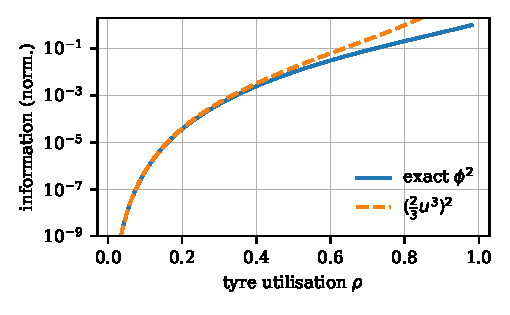
\includegraphics[width=\columnwidth]{fig1_information.pdf}
\caption{Fisher information about $\mu$ per measurement versus tire utilisation, normalised to $\rho=0.98$. The series~\eqref{eq:series} matches the exact value below $\rho\approx0.5$.}
\label{fig:info}
\end{figure}

\subsection{Estimator with stabilised forgetting}
Each update first blends the information $J=P^{-1}$ and its mean with the prior $(\mu_0,J_0)$, then applies a scalar Gauss--Newton step:
\begin{align}
J_k^- &= \lambda J_{k-1}+(1-\lambda)J_0, \label{eq:jminus}\\
\mu_k^- &= \big(\lambda J_{k-1}\hat\mu_{k-1}+(1-\lambda)J_0\mu_0\big)/J_k^-, \label{eq:muminus}\\
J_k &= J_k^-+\phi_k^2/R,\quad \phi_k=\phi(\alpha_k;\mu_k^-), \label{eq:info}\\
\hat\mu_k &= \Pi\!\left[\mu_k^-+\frac{\phi_k}{J_kR}\big(y_k-h(\alpha_k;\mu_k^-)\big)\right], \label{eq:update}
\end{align}
with forgetting factor $\lambda\in(0,1)$ and $\Pi$ a projection onto admissible values. Without excitation ($\phi_k\approx0$), both $J_k\to J_0$ and $\hat\mu_k\to\mu_0$ geometrically: the estimator returns to its prior instead of winding up its covariance or keeping a stale mean. With sustained excitation, $J_k$ approaches $J_0+\bar\phi^2/(R(1-\lambda))$.

\begin{remark}\label{rem:decay}
After strong excitation the information can exceed $J_0$ by orders of magnitude, and returning to $J_0$ takes about $\ln(J_{\mathrm{peak}}/J_0)/(1-\lambda)$ samples. With $\lambda=0.995$ at 100\,Hz and $J_{\mathrm{peak}}/J_0\approx2.7\times10^3$ this is about 16\,s---roughly 400\,m at highway speed. Time-based forgetting alone therefore cannot distinguish standing still from driving onto a new surface; this motivates the spatial term below.
\end{remark}

\subsection{Lower confidence bound}
The bound is
\begin{equation}
\mulb_k=\max\{\mu_{\min},\ \hat\mu_k-z_\delta\,J_k^{-1/2}\}, \label{eq:bound}
\end{equation}
with $z_\delta$ the one-sided Gaussian quantile for confidence $1-\delta$. The prior satisfies $\mu_0-z_\delta J_0^{-1/2}=\mu_{\min}$, so with no information the bound equals the conservative value.

\begin{remark}
Under Assumption~\ref{as:model} and small linearisation error, $\hat\mu_k$ is approximately Gaussian with variance $J_k^{-1}$, giving $\Pr(\mu\ge\mulb_k)\approx1-\delta$. This is an approximation, not a finite-sample guarantee; it fails if $c$ is wrong, noise is non-Gaussian, or $\mu$ changes within the estimator memory. Section~\ref{sec:results} measures empirical coverage.
\end{remark}

\subsection{Spatial staleness}
Let $s_{\mathrm{exc}}$ be the last position at which a measurement was informative, $\phi_k^2/R>I_{\mathrm{th}}$. The planner uses
\begin{equation}
\mu_{\mathrm{plan}}(s)=\mu_{\min}+(\mulb_k-\mu_{\min})\,e^{-(s-s_{\mathrm{exc}})/\ell}, \label{eq:decay}
\end{equation}
so trust in the bound decays with distance from where the surface was last observed, with length scale $\ell$. Anchoring at $s_{\mathrm{exc}}$ rather than the current position matters: a decay anchored at the vehicle moves with it and never reaches the curve.

% ------------------------------------------------------------
\section{Speed Planning on the Friction Bound}
On a grid $s_i$ with spacing $\Delta s$ over a horizon $H$, the planner computes the curvature limit $v_i^{\kappa}=\min\{v_{\max},\sqrt{\eta\mu_{\mathrm{plan},i}g/|\kappa_i|}\}$, a forward pass $v_{i+1}\le\sqrt{v_i^2+2a_{x,i}^{\max}\Delta s}$ with $a_{x,i}^{\max}=\min\{a_{\mathrm{acc}},\sqrt{(\eta\mu_{\mathrm{plan},i}g)^2-(v_i^2\kappa_i)^2}\}$, and a backward pass with the full braking capacity, taking the pointwise minimum as in \cite{kapania2016}. The terminal speed is limited so that the vehicle can stop within 30\,m under $\mu_{\min}$, keeping each plan recoverable if the bound drops. The plan is recomputed at 5\,Hz.

\begin{proposition}[Conditional feasibility]\label{prop:feas}
If the true friction satisfies $\mu(s)\ge\mu_{\mathrm{plan}}(s)$ over the planning horizon, the planned profile satisfies~\eqref{eq:circle} at every grid point.
\end{proposition}
\begin{proof}
By construction each planned point satisfies $\sqrt{a_{x,i}^2+a_{y,i}^2}\le\eta\mu_{\mathrm{plan},i}g\le\eta\mu(s_i)g$.
\end{proof}
The result is deterministic; the probabilistic content lies in whether $\mu\ge\mu_{\mathrm{plan}}$. Discretisation and tracking error are absorbed by $\eta$.


% ------------------------------------------------------------
\section{Simulation Study}
\subsection{Plant, controller and sensing}
The plant is a planar dynamic bicycle model (states $X,Y,\psi,v_x,v_y,r$) with the tire model~\eqref{eq:tire} on both axles, a friction ellipse reducing lateral capacity to $\sqrt{\mu^2-(a_x/g)^2}$, longitudinal acceleration saturated at $0.95\mu g$, steering lag $\tau_\delta$ and steering-rate limit, integrated by forward Euler at 100\,Hz. Steering uses curvature feedforward with preview plus heading and Stanley-type lateral feedback; speed uses feedforward plus proportional feedback. The estimator receives~\eqref{eq:force} computed from the plant's $a_y$ and $\dot r$, with Gaussian noise $\sigma_y=0.02$ on $y$ and $\sigma_\alpha=0.1^\circ$ on $\alpha$. In each run the true stiffness of both axles is scaled by a factor drawn uniformly from $[0.9,1.1]$ while the estimator keeps the nominal $c$, so model mismatch is present throughout. Parameters are in Table~\ref{tab:params}.

\begin{table}[t]
\centering\footnotesize
\caption{Simulation parameters}
\label{tab:params}
\setlength{\tabcolsep}{3pt}
\begin{tabular}{ll}
\toprule
Vehicle & $m=1500$\,kg, $I_z=2500$\,kg\,m$^2$, $l_f=1.2$, $l_r=1.6$\,m\\
 & $C_f=80$, $C_r=100$\,kN/rad, $\delta_{\max}=30^\circ$, $60^\circ$/s, $\tau_\delta=0.08$\,s\\
Estimator & $\lambda=0.995$ (100\,Hz), $\mu_0=0.6$, $\mu_{\min}=0.3$, $z_\delta=1.645$\\
Planner & $\eta=0.85$, $H=250$\,m, $\Delta s=2$\,m, $v_{\max}=25$\,m/s\\
 & $a_{\mathrm{acc}}=3$\,m/s$^2$, $\ell=150$\,m, $I_{\mathrm{th}}=1$\\
\bottomrule
\end{tabular}
\end{table}

\subsection{Track and scenarios}
All scenarios share one 1134\,m track: an 80\,m straight, a $90^\circ$ left and a $90^\circ$ right curve (radius 60\,m) separated by 80\,m, a 420\,m straight, a $120^\circ$ left test curve (radius 60\,m) and a 120\,m straight, with 20\,m clothoid transitions; the vehicle starts at 10\,m/s.
\textbf{S1 (hidden drop):} $\mu=0.9$, dropping to $0.4$ 60\,m into the long straight. \textbf{S2:} $\mu=0.35$ throughout. \textbf{S3:} $\mu=0.9$ throughout.

\subsection{Methods and metrics}
\textbf{B1} fixed $\mu=0.9$; \textbf{B2} fixed $\mu=\mu_{\min}$; \textbf{B3} certainty-equivalent, planning with $\hat\mu$; \textbf{B4} estimate minus a fixed margin, $\hat\mu-m$ with $m=0.2$; \textbf{A1} the bound without forgetting ($\lambda=1$); \textbf{A2} the bound without spatial staleness ($\ell\to\infty$); \textbf{P} proposed. All share the track, controller, $\eta$, noise seeds and stiffness draws.
Metrics: \emph{saturation time}, total time with either axle above 95\% utilisation; \emph{departure}, lateral error above 2\,m; traversal time; \emph{coverage}, fraction of time with true $\mu$ at the vehicle $\ge\mulb$. Each configuration is run with 20 seeds; we report means with 95\% confidence intervals and a Wilcoxon signed-rank test on paired saturation times.

% ------------------------------------------------------------
\section{Results}\label{sec:results}
\begin{table}[t]
\centering\small
\caption{Monte Carlo results (20 runs, mean $\pm$ 95\% CI). Sat.: tire-saturation time; Dep.: runs with lane departure; Time: traversal time (not meaningful for runs that departed); Cov.: bound coverage.}
\label{tab:main}
\setlength{\tabcolsep}{3pt}
\begin{tabular}{lcccc}
\toprule
Method & Sat.\ [s] & Dep.\ [\%] & Time [s] & Cov.\\
\midrule
\multicolumn{5}{l}{\textit{S1 hidden drop}}\\
B1 Fixed-nominal & 17.8$\pm$0.0 & 100 & 56.3$\pm$0.0 & --\\
B2 Fixed-conservative & 0.0$\pm$0.0 & 0 & 69.2$\pm$0.0 & --\\
B3 Certainty-equivalent & 31.5$\pm$3.2 & 100 & 73.5$\pm$3.3 & --\\
B4 Estimate minus margin & 0.0$\pm$0.0 & 0 & 61.2$\pm$1.2 & --\\
A1 No forgetting & 17.7$\pm$0.1 & 100 & 59.7$\pm$0.3 & 0.36\\
A2 No spatial decay & 8.0$\pm$1.7 & 60 & 57.5$\pm$0.2 & 0.61\\
Proposed & 0.2$\pm$0.1 & 0 & 58.6$\pm$0.4 & 0.54\\
\midrule
\multicolumn{5}{l}{\textit{S2 low friction}}\\
B1 Fixed-nominal & 64.3$\pm$0.0 & 100 & 69.7$\pm$0.0 & --\\
B2 Fixed-conservative & 0.0$\pm$0.0 & 0 & 69.2$\pm$0.0 & --\\
B3 Certainty-equivalent & 89.8$\pm$5.4 & 100 & 98.0$\pm$5.6 & --\\
B4 Estimate minus margin & 0.1$\pm$0.2 & 0 & 68.5$\pm$0.1 & --\\
A1 No forgetting & 1.3$\pm$0.7 & 0 & 66.7$\pm$0.4 & 0.59\\
A2 No spatial decay & 0.7$\pm$0.5 & 0 & 66.9$\pm$0.4 & 0.84\\
Proposed & 0.6$\pm$0.4 & 0 & 67.1$\pm$0.4 & 0.84\\
\midrule
\multicolumn{5}{l}{\textit{S3 high friction}}\\
B1 Fixed-nominal & 0.0$\pm$0.0 & 0 & 51.0$\pm$0.0 & --\\
B2 Fixed-conservative & 0.0$\pm$0.0 & 0 & 69.2$\pm$0.0 & --\\
B3 Certainty-equivalent & 0.3$\pm$0.2 & 0 & 51.8$\pm$0.4 & --\\
B4 Estimate minus margin & 0.0$\pm$0.0 & 0 & 57.4$\pm$2.0 & --\\
A1 No forgetting & 0.0$\pm$0.0 & 0 & 54.9$\pm$0.5 & 0.57\\
A2 No spatial decay & 0.8$\pm$0.3 & 0 & 52.9$\pm$0.4 & 0.75\\
Proposed & 0.0$\pm$0.0 & 0 & 56.2$\pm$0.8 & 0.76\\
\bottomrule
\end{tabular}
\end{table}

\begin{figure}[t]
\centering
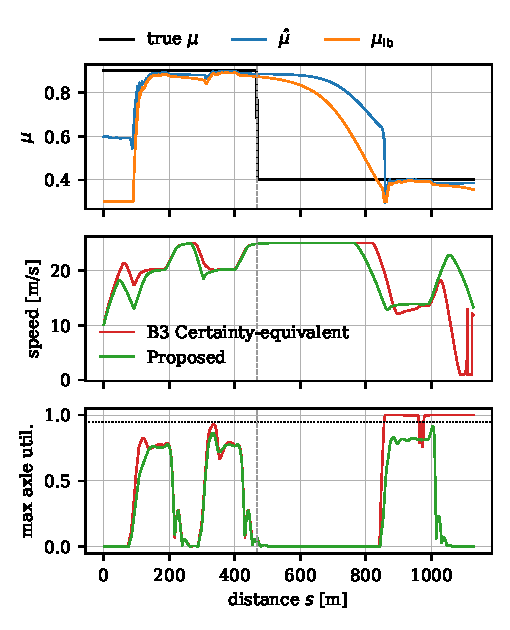
\includegraphics[width=\columnwidth]{fig2_s1_timeseries.pdf}
\caption{Scenario S1, one run. Top: true friction, estimate and bound (proposed). Middle and bottom: speed and maximum axle utilisation for certainty-equivalent planning (B3) and the proposed method. The dashed line marks the friction drop.}
\label{fig:s1}
\end{figure}

\textbf{Hidden drop (S1).} Table~\ref{tab:main} and Fig.~\ref{fig:s1} show the central failure of certainty equivalence: after converging to $\hat\mu\approx0.9$ in the first curves, B3 sees no excitation on the straight, keeps planning for high friction, and enters the test curve at 25\,m/s on $\mu=0.4$; every run saturates the tires (31.5\,s) and departs. Fixed-nominal planning (B1) and the bound without forgetting (A1) fail the same way. Without spatial staleness (A2) the bound decays too slowly (Remark~\ref{rem:decay}) and 60\% of runs depart. The proposed method brakes before the curve, saturates for $0.2\pm0.1$\,s and never departs; the difference from B3 is significant ($p=1.9\times10^{-6}$). It is 10.6\,s faster than the conservative B2.

\begin{table}[t]
\centering\footnotesize
\caption{S1 with different friction after the drop (20 runs): lane departures [\%] / mean traversal time [s].}
\label{tab:wet}
\setlength{\tabcolsep}{3pt}
\begin{tabular}{lcccc}
\toprule
Method & $\mu=0.5$ & $\mu=0.4$ & $\mu=0.33$ & $\mu=0.3$\\
\midrule
B4, $m=0.2$ & 0 / 61.7 & 0 / 62.2 & 15 / 62.8 & 70 / 67.6\\
B4, $m=0.3$ & 0 / 64.3 & 0 / 64.5 & 0 / 64.5 & 0 / 64.5\\
\textbf{Proposed} & \textbf{0 / 57.7} & \textbf{0 / 58.9} & \textbf{0 / 60.1} & \textbf{0 / 60.4}\\
\bottomrule
\end{tabular}
\end{table}

\textbf{Fixed safety margin.} A margin on the estimate (B4) is the natural alternative to an information-aware bound. With $m=0.2$ it is safe in all three scenarios of Table~\ref{tab:main} but 2.6, 1.4 and 1.2\,s slower than the proposed method. The margin works in S1 only because the estimate relaxes to the prior $\mu_0=0.6$ on the straight and $0.6-0.2$ matches the wet friction. Table~\ref{tab:wet} varies the friction after the drop: $m=0.2$ departs in 15\% and 70\% of runs at $\mu=0.33$ and $0.3$, while $m=0.3$ is safe but 4.1--6.6\,s slower than the proposed method, which is safe and fastest at every level. No single fixed margin is both safe and fast, because the margin needed depends on what has actually been observed.

\textbf{Persistent low friction (S2).} B3 starts from the prior mean $\mu_0=0.6$ and overestimates friction until the tires saturate, leading to departures in every run. The bound-based methods stay near the limit with less than 1.5\,s of saturation and are 2--2.5\,s faster than B2.

\textbf{Cost of conservatism (S3).} On high friction the proposed method needs $56.2\pm0.8$\,s versus 51.0\,s for B1 and 69.2\,s for B2, recovering 71\% of the gap. The remaining loss arises because the bound relaxes on straights and must be re-earned at each curve entry.


\textbf{Trade-off and staleness length.} Sweeping $\ell$ (10 seeds) gives S3 times of 56.7, 55.2, 54.6 and 53.9\,s for $\ell=50,100,150,300$\,m with zero S1 saturation in all four, while $\ell\to\infty$ gives 52.7\,s but 7.6\,s of S1 saturation; $\ell$ is a tunable trust distance with a wide safe range in this setup.

\textbf{Coverage and stiffness mismatch.} Coverage is below the nominal 95\% in every scenario (Table~\ref{tab:main}). In S1 this is expected, since safety after the drop comes from spatial staleness rather than from the bound; in S2 and S3 it is caused by stiffness mismatch. Sweeping the true-to-model stiffness ratio (10 seeds each) shows the mechanism: at 0.8, 0.9 and 1.0 coverage in S2 is $\ge0.999$ with no saturation, but at 1.1 coverage falls to 0.59 with 2.9\,s of saturation, and at 1.2 the method overestimates friction and saturates for 69\,s. A stiffer-than-modelled tire produces more force at a given slip, which the estimator attributes to higher friction. A model stiffness above the true value therefore makes the bound conservative, while a model stiffness below the true value is the main failure mode.

\subsection{Validation in CARLA}
\begin{figure}[t]
\centering
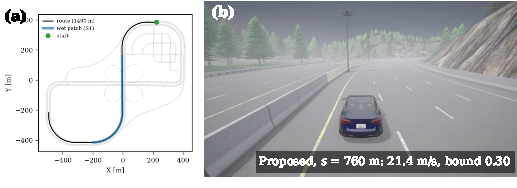
\includegraphics[width=\columnwidth]{fig_carla_scene.pdf}
\caption{CARLA experiment. (a) Town04 route (1490\,m) and S1 wet patch. (b) Chase view of the proposed planner entering the wet curve after its bound has decayed.}
\label{fig:scene}
\end{figure}

\textbf{Setup.} We repeated S1 and S3 in CARLA 0.9.16 \cite{dosovitskiy2017} with a Tesla Model~3 on a 1490\,m Town04 highway route without junction turns (minimum radius 165\,m, Fig.~\ref{fig:scene}). Axle distances were computed from the wheel positions ($l_f=1.168$, $l_r=1.836$\,m); the speed-dependent steering reduction was disabled; steering uses pure pursuit with look-ahead $\max(8\,\mathrm{m},\,v\cdot1\,\mathrm{s})$ and speed a PI loop whose throttle is reduced with lateral acceleration. The normalised stiffness was identified from linear-region data as $c=14.5$ (90\% interval 14.51--14.56) and the upper value was used. Friction was set through CARLA's \emph{tire\_friction} parameter: 1.0 for the road and 0.6 for a wet patch that starts 60\,m into the longest straight and ends after the following curve (S1). The speed limit was 30\,m/s. CARLA runs are not bit-reproducible even with a fixed seed, so we report 5 runs per configuration and treat the outcomes as samples.

\textbf{Controller acceptance and usable grip.} To separate controller limitations from planning decisions, the low-level controller was frozen after an acceptance test: fixed planning friction 0.5 and 0.6 (peak planned lateral acceleration 0.43 and 0.51\,g) completed the dry route in all runs, while 0.7 (0.60\,g) left the lane in every run. Together with a tyre-curve fit ($\mu\approx0.69$), this places the usable dry friction at about 0.6--0.7; the same fit gives about 0.33 on the wet patch.

\begin{table}[t]
\centering\footnotesize
\caption{CARLA results (5 runs each): departures [\%] and mean time of finished runs [s].}
\label{tab:carla}
\setlength{\tabcolsep}{2.5pt}
\begin{tabular}{lcccc}
\toprule
 & \multicolumn{2}{c}{S1 wet patch} & \multicolumn{2}{c}{S3 dry}\\
Method & Dep.\ [\%] & Time [s] & Dep.\ [\%] & Time [s]\\
\midrule
B1 Fixed-nominal & 100 & -- & 100 & --\\
B2 Fixed-conservative & 0 & 70.1 & 0 & 70.1\\
B3 Certainty-equivalent & 100 & -- & 100 & --\\
B4 Estimate minus margin & 0 & 68.3 & 60 & 67.9\\
A1 No forgetting & 0 & 67.7 & 0 & 67.5\\
A2 No spatial decay & 0 & 68.0 & 40 & 67.9\\
\textbf{Proposed} & \textbf{0} & \textbf{68.2} & \textbf{0} & \textbf{68.2}\\
\bottomrule
\end{tabular}
\end{table}

\begin{figure}[t]
\centering
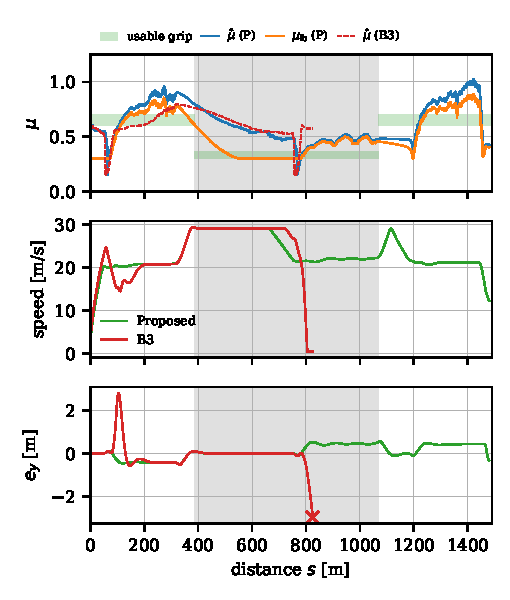
\includegraphics[width=\columnwidth]{fig4_carla_s1.pdf}
\caption{CARLA, scenario S1 (grey: wet patch; green bands: usable grip). Top: estimate and bound of the proposed method, and the certainty-equivalent estimate (B3). Middle and bottom: speed and lateral error. Both estimates are similar at the end of the straight, but only the bound has decayed, so only the proposed planner slows before the wet curve; B3 enters at 26.6\,m/s and leaves the lane (cross).}
\label{fig:carla}
\end{figure}

\textbf{Results.} Table~\ref{tab:carla} shows that the proposed method was the only adaptive planner without departures in both scenarios and was 1.8\,s (2.6\%) faster than the fixed conservative planner. Fixed-nominal planning ($\mu=0.9$) exceeded the usable grip and departed in every run. Certainty-equivalent planning departed in every run, nine times in the first curve, and in 7 of 8 additional S1 runs, all in the first curve: its speed plan followed the estimate at curve entry, which first dropped to about 0.2 and then rose to 0.65--0.71, at or above the usable grip, so the vehicle entered the curve accelerating and lost the rear axle. In the remaining run (Fig.~\ref{fig:carla}) B3 reached the end of the straight with $\hat\mu\approx0.53$, kept 29\,m/s until 740\,m and entered the wet curve at 26.6\,m/s, demanding about 0.58\,g against roughly 0.33\,g available; the proposed planner, whose bound had decayed to 0.30, slowed to 21\,m/s first. Without spatial staleness (A2), the bound reached 0.80--0.82 on the dry road and the vehicle departed in 2 of 5 runs; the fixed margin (B4) departed in 3 of 5 dry runs at the same curve, because subtracting 0.2 from an overestimated friction still left the plan at or above the usable grip.

\textbf{Two differences from simulation.} First, the estimator \emph{overestimated} dry friction in CARLA ($\hat\mu$ 0.77--0.94 against a usable 0.6--0.7), which we attribute to the mismatch between the $\tanh$ model~\eqref{eq:tire} and CARLA's tyre model; the proposed method remained safe because of spatial staleness and the factor $\eta$, not because the bound was correct, so the coverage interpretation of~\eqref{eq:bound} does not carry over. Second, the vehicle cornered at only 30--45\% of the usable grip, so by~\eqref{eq:series} the estimators accumulated little information and never became confident; consequently the ablation without forgetting (A1) did not fail, unlike in simulation. Both are consistent with Section~IV: staleness is dangerous in proportion to the excitation that produced the estimate, and the bound is only as good as the tyre model.

% ------------------------------------------------------------
\section{Discussion and Limitations}
The main quantitative results are from a simplified simulation, and the CARLA study shows that model mismatch can make the bound overconfident: a point-mass friction circle, static axle loads, ideal sensing of $a_y$ and $\dot r$ with additive noise, and a tire model whose shape the estimator knows. The most important limitation is the dependence on $c$: the bound is only as trustworthy as the stiffness model, and a conservative (higher) model stiffness, or joint estimation of $c$ in the linear region, should be used in practice. The spatial staleness model~\eqref{eq:decay} is a design choice, not derived from road statistics; map or camera-based surface priors could replace it. Finally, the planner is passive: it never deliberately excites the tires. Planning for information---trading a small excitation manoeuvre for a tighter bound---is a dual-control problem and a direction for future work.

\section{Conclusion}
For a saturating tire model, information about friction grows with the sixth power of tire utilisation, so ordinary driving leaves friction largely unidentified. An excitation-aware lower confidence bound with stabilised forgetting and spatial staleness, used in a friction-circle speed planner, removed tire saturation and lane departures after a hidden friction drop in simulation, where certainty-equivalent planning failed in every run, while recovering 71\% of the speed lost by fixed conservative planning; in CARLA it was the only adaptive planner without departures. The method is sensitive to underestimating tire stiffness in the model, which must be addressed before deployment.

\section*{Acknowledgment}
The author used an AI assistant (Claude, Anthropic) to help formulate the estimator and planner, write the simulation and CARLA code, draft the manuscript text and produce the figures. The author ran all experiments, verified the code, results and text, and takes full responsibility for the content.

\begin{thebibliography}{99}
\footnotesize
\bibitem{gustafsson1997} F.~Gustafsson, ``Slip-based tire--road friction estimation,'' \emph{Automatica}, vol.~33, no.~6, pp.~1087--1099, 1997.
\bibitem{hahn2002} J.-O.~Hahn, R.~Rajamani, and L.~Alexander, ``GPS-based real-time identification of tire--road friction coefficient,'' \emph{IEEE Trans.\ Control Syst.\ Technol.}, vol.~10, no.~3, pp.~331--343, 2002.
\bibitem{khaleghian2017} S.~Khaleghian, A.~Emami, and S.~Taheri, ``A technical survey on tire--road friction estimation,'' \emph{Friction}, vol.~5, no.~2, pp.~123--146, 2017.
\bibitem{brown2017} M.~Brown, J.~Funke, S.~Erlien, and J.~C.~Gerdes, ``Safe driving envelopes for path tracking in autonomous vehicles,'' \emph{Control Eng.\ Pract.}, vol.~61, pp.~307--316, 2017.
\bibitem{funke2017} J.~Funke, M.~Brown, S.~M.~Erlien, and J.~C.~Gerdes, ``Collision avoidance and stabilization for autonomous vehicles in emergency scenarios,'' \emph{IEEE Trans.\ Control Syst.\ Technol.}, vol.~25, no.~4, pp.~1204--1216, 2017.
\bibitem{christ2021} F.~Christ, A.~Wischnewski, A.~Heilmeier, and B.~Lohmann, ``Time-optimal trajectory planning for a race car considering variable tyre--road friction coefficients,'' \emph{Veh.\ Syst.\ Dyn.}, vol.~59, no.~4, pp.~588--612, 2021.
\bibitem{svensson2022} L.~Svensson \emph{et al.}, ``Traction adaptive motion planning and control at the limits of handling,'' \emph{IEEE Trans.\ Control Syst.\ Technol.}, vol.~30, no.~5, p.~1888, 2022.
\bibitem{iarc2026} Y.~Zhou \emph{et al.}, ``Online constraint optimization-based indirect-adaptive robust control for autonomous vehicles with unknown friction,'' arXiv:2610.22675, 2026.
\bibitem{bergerhoff2026} T.~Bergerhoff, S.~Baader, P.~Mei\ss ner, and F.~Deinzer, ``Pushing the performance limits in autonomous racing: Continuous stability-aware adaptive velocity planning in Formula Student Driverless,'' arXiv:2606.10733, 2026.
\bibitem{kapania2016} N.~R.~Kapania, J.~Subosits, and J.~C.~Gerdes, ``A sequential two-step algorithm for fast generation of vehicle racing trajectories,'' \emph{J.\ Dyn.\ Syst.\ Meas.\ Control}, vol.~138, no.~9, 2016.
\bibitem{ljung1999} L.~Ljung, \emph{System Identification: Theory for the User}, 2nd~ed. Prentice Hall, 1999.
\bibitem{astrom1995} K.~J.~{\AA}str\"om and B.~Wittenmark, \emph{Adaptive Control}, 2nd~ed. Addison-Wesley, 1995.
\bibitem{narendra1989} K.~S.~Narendra and A.~M.~Annaswamy, \emph{Stable Adaptive Systems}. Prentice Hall, 1989.
\bibitem{kulhavy1993} R.~Kulhav\'y and M.~B.~Zarrop, ``On a general concept of forgetting,'' \emph{Int.\ J.\ Control}, vol.~58, no.~4, pp.~905--924, 1993.
\bibitem{abbasi2011} Y.~Abbasi-Yadkori, D.~P\'al, and C.~Szepesv\'ari, ``Improved algorithms for linear stochastic bandits,'' in \emph{Adv.\ Neural Inf.\ Process.\ Syst.}, 2011, pp.~2312--2320.
\bibitem{dosovitskiy2017} A.~Dosovitskiy, G.~Ros, F.~Codevilla, A.~L\'opez, and V.~Koltun, ``CARLA: An open urban driving simulator,'' in \emph{Proc.\ Conf.\ Robot Learn.}, 2017, pp.~1--16.
\end{thebibliography}

\end{document}
